\documentclass[a4paper]{article}
\usepackage[affil-it]{authblk}
\usepackage[backend=bibtex,style=numeric]{biblatex}
\usepackage{ctex}
\usepackage{graphicx}
\usepackage{subcaption}
\usepackage{float} 
\usepackage{xcolor}
\usepackage{amsmath}
\usepackage{geometry}
\usepackage{amssymb}
\usepackage{mathtools}
\geometry{margin=1.5cm, vmargin={0pt,1cm}}
\setlength{\topmargin}{-1cm}
\setlength{\paperheight}{29.7cm}
\setlength{\textheight}{25.3cm}

\addbibresource{citation.bib}

\begin{document}
% =================================================
\title{Numerical Analysis homework 1}

\author{Lingxi Gao 3210105373
  \thanks{Electronic address: \texttt{3210105373@zju.edu.cn}}}
\affil{(mathematics and applied mathematics 2102 ), Zhejiang University }


\date{Due time: 24/10/7}

\maketitle






% ============================================
\section*{代码设计思路}
我编写的代码是一个用于求解非线性方程根的 C++ 程序,它实现了三种经典的数值求解方法:二分法(Bisection Method)、牛顿法(Newton Method) 和 割线法(Secant Method)。所有这些方法都被设计成类,每个类继承自一个基类 EquationSolver。此外我的程序用差商近似导数,具体的公式为${f}'(x)=\frac{f(x+10^{-6})-f(x)}{10^{-6}}$


\section*{C++ Program Output}

\begin{verbatim}
	Running program_B...
	./program_B
	the root of x^{-1}-tan(x) on [0,pi/2] is 0.860333
	the root of 1/x-2^x  on [0,1]is  0.641186
	the root of 2^{-x}+e^x+2cosx-6 on [1,3]  is  1.82938
	the root of (x^3+4x^2+3x+5)/(2x^3-9x^2+18x-2) is  0.117876
	Running program_C...
	./program_C
	Solving x - tan x near 4.5
	A root is: 4.49341
	Solving x - tan x near 7.7
	A root is: 7.72525
	Running program_D...
	./program_D
	the root of sin(x/2)-1  with x0=0 x1=pi/2 is  3.14144
	the root of sin(x/2)-1  with x0=pi/2 x1=pi is  3.14159
	the root of e^x-tanx with x0=1,x1=1.4 is  1.30633
	the root of e^x-tanx with x0=0.5,x1=1.4 is  -6.28131
	the root of x^3-12x^2+3x+1  with x0=0, x1=-0.5 is -0.188685
	the root of x^3-12x^2+3x+1  with x0=-1.5, x1=-1.0 is  -0.188685
	Running program_E...
	./program_E
	the height of water is 0.84375
	the height of water is 0.833834
	the height of water is 0.833834
	Running program_F...
	./program_F
	(a) under the condition, alpha is 
	32.9722 degree
	(b) under the condition, alpha is 
	33.1689 degree
	(c) under the condition, alpha is 
	-11.5 degree
	(c) under the condition, alpha is 
	168.5 degree
	
	
\end{verbatim}
\section*{分析}
\subsection{problem B}
由于(1)(2)两问中两个函数在0处有极点,因此带入二分法程序求解零点时,应当适当缩小初始区间,避免出现函数值无穷大的情况使二分法失效。(4)中有理函数分母在区间$[0,4]$上分母有零点,显然二分法的程序没有找到该函数真正的零点,该函数在$[0,4]$上也没有零点。导致程序停止的原因可能是迭代次数已达到最大值。因此在使用二分法时选择初始区间时应当注意避开分母可能为零的点。

\subsection{problem C}
从C的结果可以看出,当函数有多个零点时,使用牛顿法求根会依赖初值的选择,牛顿法倾向于找到更接近初值的零点。

\subsection{problem D}
从D的结果可以看出,割线法同样收初值的选取影响很大。(1)的结果能够看出,当函数零点不唯一时,割线法会收敛到靠近初始区间的零点。


(2)中结果看出割线法有一定的不稳定性,尽管初值给的区间在正半轴上,收敛的结果仍然是位于负半轴上里初始区间更远的零点。绘制出$f(x)=e^x-tan x$在区间$[0.5,1.4]$上的图像。从图像中能看出,$f(x)=e^x-tan x$在区间$[0.5,1]$上函数值变化非常小,因此根据割线法的迭代公式$x_{n+1}=x_n-f(x_n)\frac{x_n-x_{n-1}}{f(x_n)-f(x_{n-1})}$可知,$\frac{x_n-x_{n-1}}{f(x_n)-f(x_{n-1})}$会很大,因此求得的零点会距离初始区间比较远。而$f(x)=e^x-tan x$在$[1,1.4]$上函数值变化较快,因此使用割线法得到的零点也会接近初始区间。因此在使用割线法求解函数零点时,也要注意函数在初始区间上的变化幅度。(本题图像见下一页)
\vfill  % 空出页面中剩余空间,推动图片到页面底部

% 插入图片在第一页底端,并调整大小
\begin{figure}[H]  % 使用b选项确保图片在页面底部
	\centering
	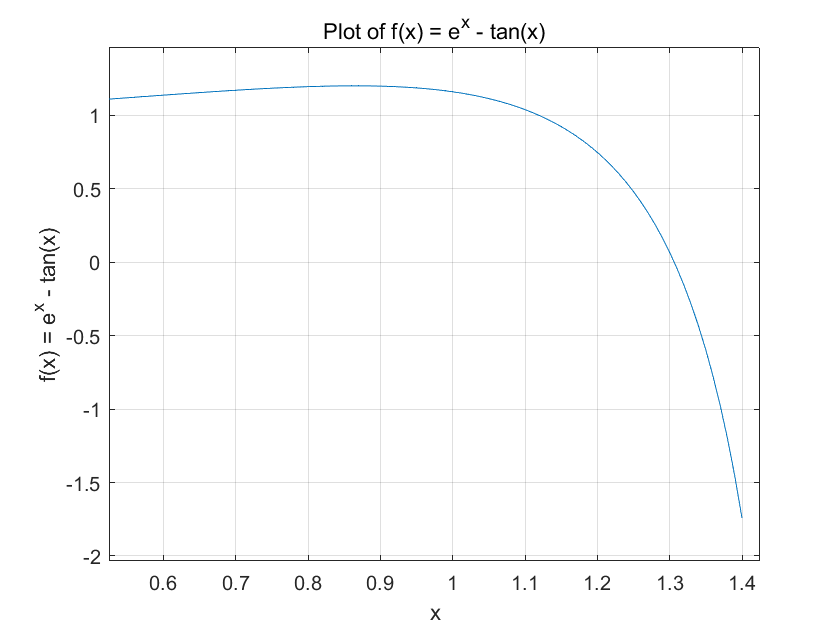
\includegraphics[width=0.5\textwidth]{f1.png}  % 调整图片宽度
	\caption{Plot of $f(x) = e^x - \tan(x)$ in the interval $[0.5, 1.4]$}
	\label{fig:function_plot}
\end{figure}

(3)中函数为$f(x)=x^3-12x^3+3x+1$。从图像中可以看出$f$在$[-1.5,-1.0]$上没有零点,但割线法仍然收敛到了$[-1.0,0]$上的零点,$f$在$[-1.5,-1.0]$上斜率没有过大和过小。


综合(1)(2)(3)问可以看出,割线法依赖与初始区间的选择,当函数的斜率在一段测度不为0的集合上不接近0时,割线法会收敛到初始区间附近的零点,此时结果会比较理想。但是当函数斜率在一个区间上很接近0时,割线法会不稳定,找到的零点不一定是初始区间附近的。

\begin{figure}[H]  % 使用b选项确保图片在页面底部
	\centering
	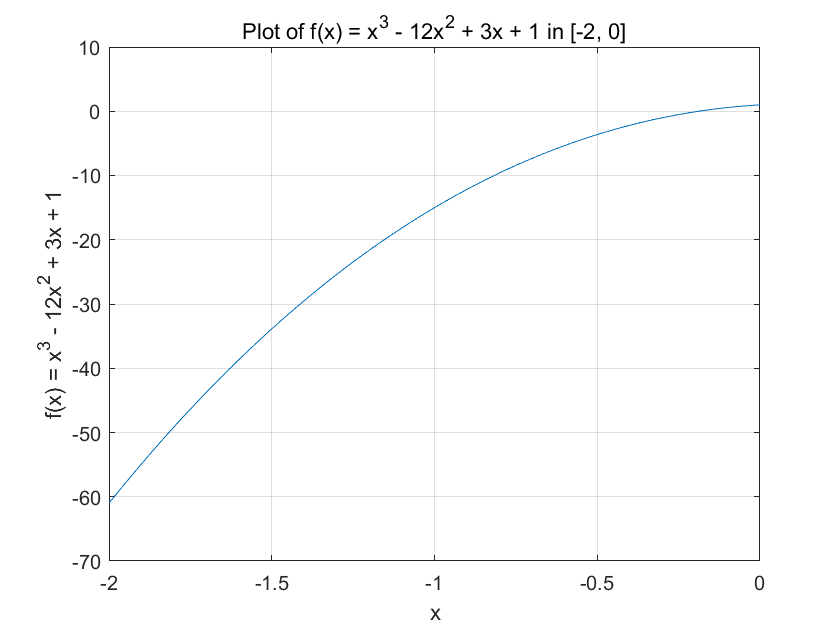
\includegraphics[width=0.5\textwidth]{f2.png}  % 调整图片宽度
	\caption{Plot of $f(x) =x^3-12x^3+3x+1$ in the interval $[-1.5, 0]$}
	\label{fig:function_plot}
\end{figure}

\subsection{problem E}
本题要求水深,我们先求图片中的h,再用1-h即可得到水深。要求迭代求出的零点和精确值之间误差小于0.01,是一种绝对误差,下面设$\alpha$为函数真正的零点,$x_0$为迭代得到的函数零点,说明E.cpp中初值的设置理由。

对于二分法:$|\alpha-x_0| \le \frac{|a_n-b_n|}{2}$,其中$[a_n,b_n]$为第n次迭代后的区间,因此只要设置停止条件为$\delta=|b_n-a_n| \le 0.01$即可满足题目要求。

对于牛顿法:在$x_n$处Taylor展开可得
$x_n-\alpha=\frac{f(x_n)}{{f}'(x_n)}+\frac{(\alpha-x_n)^2{f}''(\eta)}{2{f}'(\eta)}$
事实上根据二分法的结果显示,实际的零点应当在$[0.14,0.17]$,因此选择初值$h_0$为0.14,当迭代次数很多时$\frac{(\alpha-x_n)^2{f}''(\eta)}{2{f}'(\eta)}$会小于0.005,因此只要$\frac{f(x_n)}{{f}'(x_n)} \le 0.005$即可。通过计算,$|{f}'(x)| \le 40 \: x \in [0, 0.5]$,因此取$\epsilon$为0.00025。

对于割线法:与牛顿法一样,初值选取0.14和0.17,由定理1.25,$|x_n-\alpha| \le M|x_n-\alpha|^1.618$ 若$|x_n-\alpha| \le M(|x_{n-1}-\alpha|+|x_n-x_{n-1}|)^1.618 \le 0.01$成立,只要 $\delta=|x_n-x_{n-1}| \le \sqrt[1.618]{\frac{0.01}{M} } -0.01$即可,这里取M充分大,取为100。得到$\delta$大约为0.001。

从结果中可以看出二分法和其他两种方法的结果相差比较大。这里推测割线法和牛顿法结果相近是由于当$x_n$和$x_{n-1}$很接近时,导数和割线也很接近,因此两种方法的结果会很接近。结果的差异是由于二分法最终返回的是区间端点的值。
\subsection{problem F}
本题需要将弧度制转化为角度制。因为在此题的背景中,$\alpha$的范围只能是$0~180$度,因此(c)中另外两组初值我分别选择了3,5和170,175度。
在初值选择3和5的时候,结果出现了负数,是方程在其他区间的零点,但是没有实际应用价值。



\end{document}